% !TEX encoding = UTF-8
%Koma article
\documentclass[fontsize=12pt,paper=letter,twoside]{scrartcl}
\usepackage{float}
\usepackage{listings}
\usepackage{makecell}

%Standard Pre-amble
\usepackage[top=4cm,bottom=4cm,left=3cm,right=3cm,asymmetric]{geometry}
%\geometry{landscape}                % Activate for for rotated page geometry
%\usepackage[parfill]{parskip}    % Begin paragraphs with an empty line rather than an indent
\usepackage[table,xcdraw]{xcolor}
\usepackage{graphicx}

\usepackage{amsmath}
\usepackage{amssymb}
\usepackage{epstopdf}
\DeclareGraphicsRule{.tif}{png}{.png}{`convert #1 `dirname #1`/`basename #1 .tif`.png}
% Listings needs package courier
\usepackage{listings} % Needs 
\usepackage{courier}

\usepackage[framemethod=TikZ]{mdframed}
\usepackage{url}

\usepackage{sty/bsymb} %% Event-B symbols
\usepackage{sty/eventB} %% REQ and ENV
\usepackage{sty/calculation}

%Maths
\usepackage{amssymb,amsmath}
\def\Fl{\mathbb{F}}
\def\Rl{\mathbb{R}}
\def\Nl{\mathbb{N}}
\def\Bl{\mathbb{B}}
\def\St{\mathbb{S}}
\newcommand{\ovr}{\upharpoonright}
\newcommand{\var}[1]{\textit{#1}}
%Useful definitions
\newcommand{\mv}[1]{\textit{m\_#1}}
\newcommand{\cv}[1]{\textit{c\_#1}}
\newcommand{\degree}[1]{^{\circ}\mathrm{#1}}
%\newcommand{\comment}[1]{{\footnotesize \quad\texttt{--}\textrm{#1}}}
\newcommand{\im}[1]{i\texttt{-\!#1}}

\usepackage[headsepline]{scrpage2}
\pagestyle{scrheadings}
\ihead[]{\small EECS4312 Report1}
\ohead[]{\small \thepage}
\cfoot[]{}
\ofoot[]{}


%%%%PVS environment%%%%%%%%%%%%%%%%%%%
\lstnewenvironment{pvs}[1][]
    {\lstset{#1,captionpos=b,language=pvs,
    mathescape=true,
    basicstyle=\small\ttfamily,
    numbers=none,
    frame=single,
    % numberstyle=\tiny\color{gray},
    % backgroundcolor=\color{lightgray},
    firstnumber=auto
    }}
    {}
 %%%%%%%%%%%%%%%%%%%%%%%%%%%%%%%%
 
%%%%Verbatim environment%%%%%%%%%%%%%%%%%%%
\lstnewenvironment{code}[1][]
    {\lstset{#1,captionpos=b,
    mathescape=true,
    basicstyle=\small\ttfamily,
    numbers=none,
    frame=single,
    % numberstyle=\tiny\color{gray},
    % backgroundcolor=\color{lightgray},
    firstnumber=auto
    }}
    {}

% \newenvironment{boxed}[1]
%    {\begin{center}
%    #1\\[1ex]
%    \begin{tabular}{|p{0.9\textwidth}|}
%    \hline\\
%    }
%    { 
%    \\\\\hline
%    \end{tabular} 
%    \end{center}
%    }
 %%%%%%%%%%%%%%%%%%%%%%%%%%%%%%%%
 
 %Text in a box
\newenvironment{textbox}
    {\begin{center}
    \begin{tabular}{|p{0.9\textwidth}|}
    \hline\\
    }
    { 
    \\\\\hline
    \end{tabular} 
    \end{center}
    }

\usepackage{hyperref}

%Highlight \hl{}
\usepackage{soul}

\usepackage{enumitem}
\newlist{mylist}{itemize}{1}
\setlist[mylist]{label=\textbullet,leftmargin=1cm,nosep}

\usepackage{multirow}

% Reduce space between figure and caption
%\usepackage{caption}
%\captionsetup[table]{font=small,skip=0pt}     %% Adjust here
%or equivalently 
\usepackage[font=small,skip=4pt]{caption}
%Useful definitions
%\newcommand{\mv}[1]{\textit{m\_#1}}
%\newcommand{\cv}[1]{\textit{c\_#1}}
%\newcommand{\degree}[1]{^{\circ}\mathrm{#1}}
%\newcommand{\comment}[1]{{\footnotesize \quad\texttt{--}\textrm{#1}}}


%For Code Stylings
\usepackage{listings}
\usepackage{color}

\definecolor{dkgreen}{rgb}{0,0.6,0}
\definecolor{gray}{rgb}{0.5,0.5,0.5}
\definecolor{mauve}{rgb}{0.58,0,0.82}

\lstset{frame=tb,
  language=Java,
  aboveskip=3mm,
  belowskip=3mm,
  showstringspaces=false,
  columns=flexible,
  basicstyle={\small\ttfamily},
  numbers=none,
  numberstyle=\tiny\color{gray},
  keywordstyle=\color{blue},
  commentstyle=\color{dkgreen},
  stringstyle=\color{mauve},
  breaklines=true,
  breakatwhitespace=true,
  tabsize=3
}

% Set the header
\ihead[]{\small EECS4313 Assignment-3}


%%%%%%%%%%%%Enter your names here%%%%%%%%
\author{Student Name | Student Number | EECS Account
\and \textbf{Edward Vaisman | 212849857 | eddyv}
\and \textbf{Robin Bandzar | 212200531 | cse23028}
\and \textbf{Kirusanth Thiruchelvam | 212918298 | kirusant}
\and \textbf{Sadman Sakib Hasan | 212497509 | cse23152}
}
%%%%%%%%%%%%%%%%%%%%%%%%%%%%%%%%

\date{\today} % Display a given date or no date

\begin{document}
\title{EECS 4313 Assignment 3 \\Data Flow Testing, Slice-Based Testing and Mutation Testing}
\maketitle

\newpage

%%%%%%%%%%%%%%%%%%%%%%%%%%%%%%%
\tableofcontents


\newpage


\section{BORG Calendar}

\subsection{Mutation Testing}
Mutation tests were run using the previous unit test suite that we created for assignment 2. The program used to run the Mutation tests was \emph{Eclispe} with the \emph{Pitclipse} plugin. The three methods that we tested are listed with their results in the following subsections. 

\subsubsection{minuteString Function}


\begin{figure}[!htb]
\begin{center}
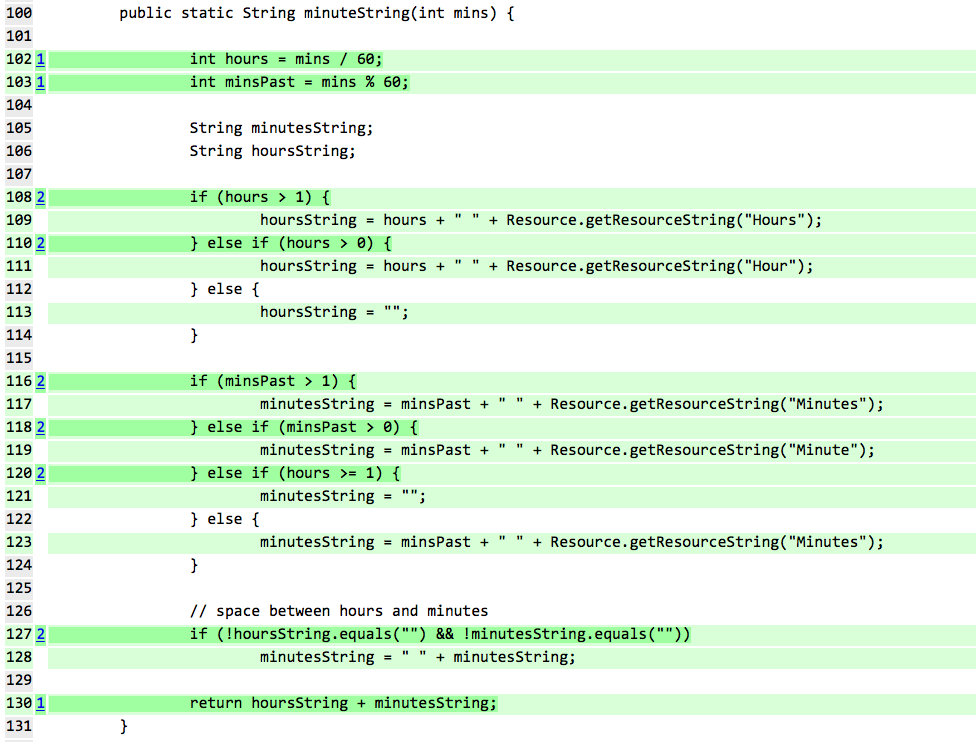
\includegraphics[width=.99\textwidth]{images/MutationTesting/minuteStringCode.png}
\end{center}
\caption{Code for the minuteString method}
\label{fig:minuteStringCode}
\end{figure}

\begin{figure}[!htb]
\begin{center}
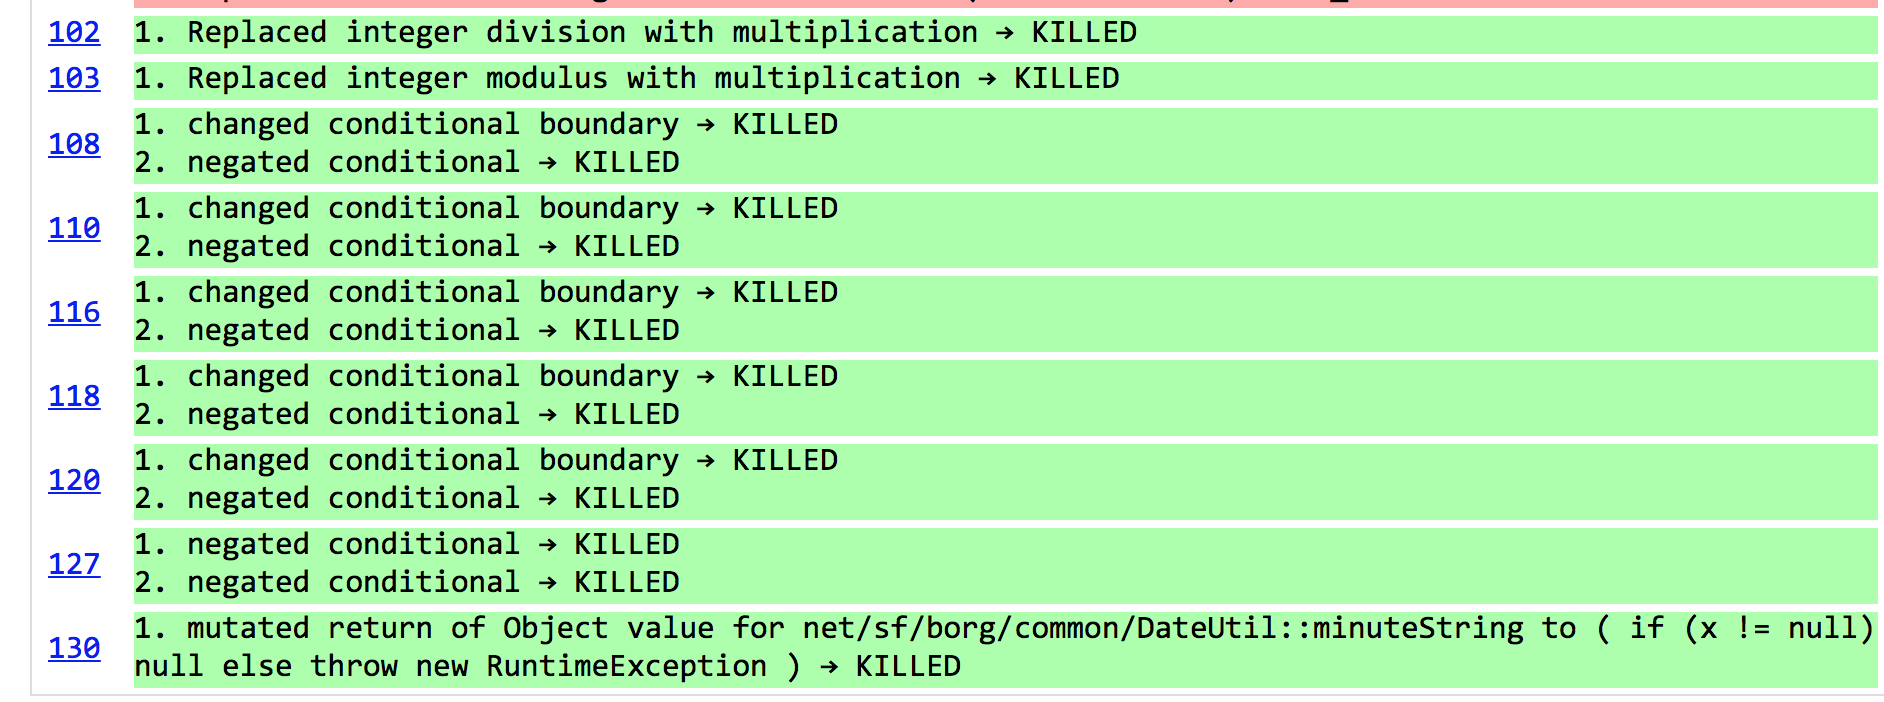
\includegraphics[width=.99\textwidth]{images/MutationTesting/minuteStringMutant.png}
\end{center}
\caption{Mutations for the minuteString method}
\label{fig:minuteStringMutant}
\end{figure}

\clearpage
As one can see in Figures \ref{fig:minuteStringCode} and \ref{fig:minuteStringMutant} that the previous tests effectively kill all the mutants so no further changes are needed.


\subsubsection{isAfter Function}
\begin{figure}[!htb]
\begin{center}
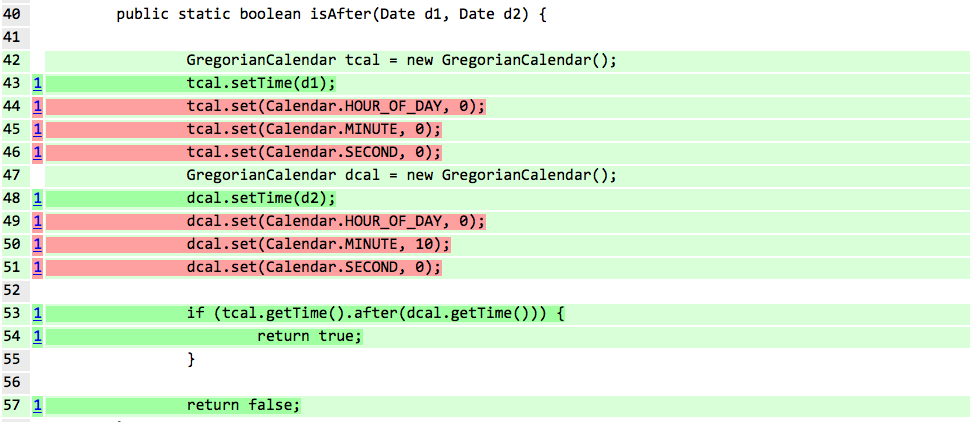
\includegraphics[width=.99\textwidth]{images/MutationTesting/isAfterCode.png}
\end{center}
\caption{Code for the isAfter method}
\label{fig:isAfterCode}
\end{figure}

\begin{figure}[!htb]
\begin{center}
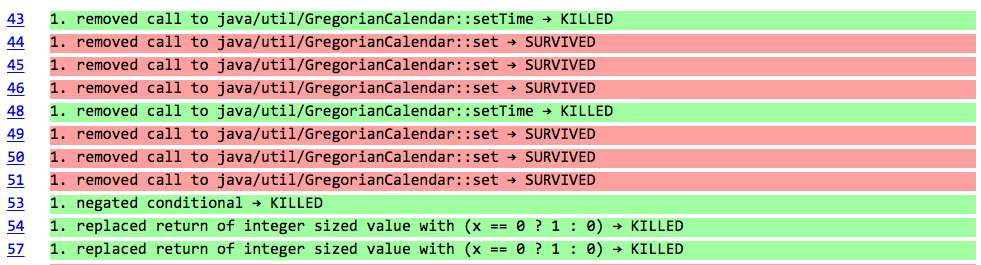
\includegraphics[width=.99\textwidth]{images/MutationTesting/isAfterMutant.png}
\end{center}
\caption{Mutations for the isAfter method}
\label{fig:isAfterMutant}
\end{figure}

\clearpage
\noindent Looking at the result of the mutation test result from Figure \ref{fig:isAfterMutant}, it is inevitable that the method \emph{isAfter} will still pass tests even after removing the lines 44-46 and 49-51. This means those lines (line 44-46 and line 49-51) can never have any affect on the expected output of the method.

\bigskip

\noindent This can be proved by adding a simple test case which creates two date objects and set their minute, hour and second to some value. No matter what value for minute, hour and second is passed with the Date object, the function will always create a Gregorian Calendar instance with values of 0 for the first date object. Similarly, it will create another Gregorian Calendar instance with values 0 for hours and seconds and 10 for minutes for the second date object.

\bigskip

\noindent \textbf{Example test case:} \label{isAfter:example_test_case}

\begin{code}
    @Test
    public void testIsAfterBug() {
    	// Both happens at the same day, but at different hours
    	// but the implementation ignores the hours, minutes
    	// and seconds
    	Date d1 = new Date( 2018 , 8 , 24 , 8 , 30 , 24 );
    	Date d2 = new Date( 2018 , 8 , 24 , 9 , 30 , 24 );
    	
    	// This works correctly. The assert returns true
    	assertFalse(DateUtil.isAfter(d1, d2));
    	// This does not work correctly. The assert returns false,
    	// when it should be true
    	assertTrue(DateUtil.isAfter(d2, d1));
    }
\end{code}

\bigskip

\noindent \textbf{Bug Report:}

\begin{itemize}
\item \textbf{Bug Report Title}: The \emph{isAfter} function ignores hours, minutes and seconds fields from the passed in date object.
\item \textbf{Reported by}: Sadman Sakib Hasan
\item \textbf{Date reported}: Saturday, March 24, 2018
\item \textbf{Program (or component) name}: BORG Calendar version 1.8.3
\item \textbf{Configuration(s)}:\\
\underline{System Info}
\begin{itemize}
\item{Operating System: Windows 10 Pro 64-bit (10.0, Build 16299)}
\item {Language: English (Regional Setting: English)}
\item {System Manufacturer: Hewlett-Packard}
\item {System Model: HP 15 TouchSmart Notebook PC}
\item {BIOS: F.10}
\item {Processor: AMD A6-5200 APU with Radeon(TM) HD Graphics (4 CPUs), ~2.0GHz }
\item {Memory: 6144MB RAM}
\item {Java Version: 1.8.0\_151-b12}
\end{itemize}
\item \textbf{Report type}: Coding Error
\item \textbf{Reproducibility}: 100\%
\item \textbf{Severity}: Medium
\item \textbf{Problem summary}: The \emph{isAfter} method automatically sets the HOUR\_OF\_DAY, MINUTE, and SECOND values of the newly created Gregorian Calendar object from the passed in dates d1 and d2 to a constant value.
\item \textbf{Problem description}: The \emph{isAfter} method in \emph{net.sf.borg.common.DateUtil} does not take into account the hours, minutes, and seconds of the given date objects when comparing the two dates. A newly Gregorian Calendar object is created for both argument, d1 and d2, and the hours, minutes and seconds are set to 0 for \emph{d1}'s calendar instance whereas the hours and seconds are set to 0 and minute set to 10 for \emph{d2}'s calendar instance. This causes an issue when there are comparison between two dates that are in the same day, and hours, minutes and seconds differ as shown in the example test case \ref{isAfter:example_test_case}.
\item \textbf{Steps to Reproduce}:
\begin{itemize}
\item Create two date objects, d1 and d2, with the day set to the same value and hours, minutes and seconds set to different values.
\item Compare the two dates using \emph{isAfter} function.
\item The \emph{isAfter} function will always return false regardless of the fact if d1 is ahead on hours/minutes/seconds or vice versa.
\end{itemize}
\item \textbf{New or old bug}: New
\end{itemize}


\subsubsection{sendMsg Function}
\begin{figure}[!htb]
\begin{center}
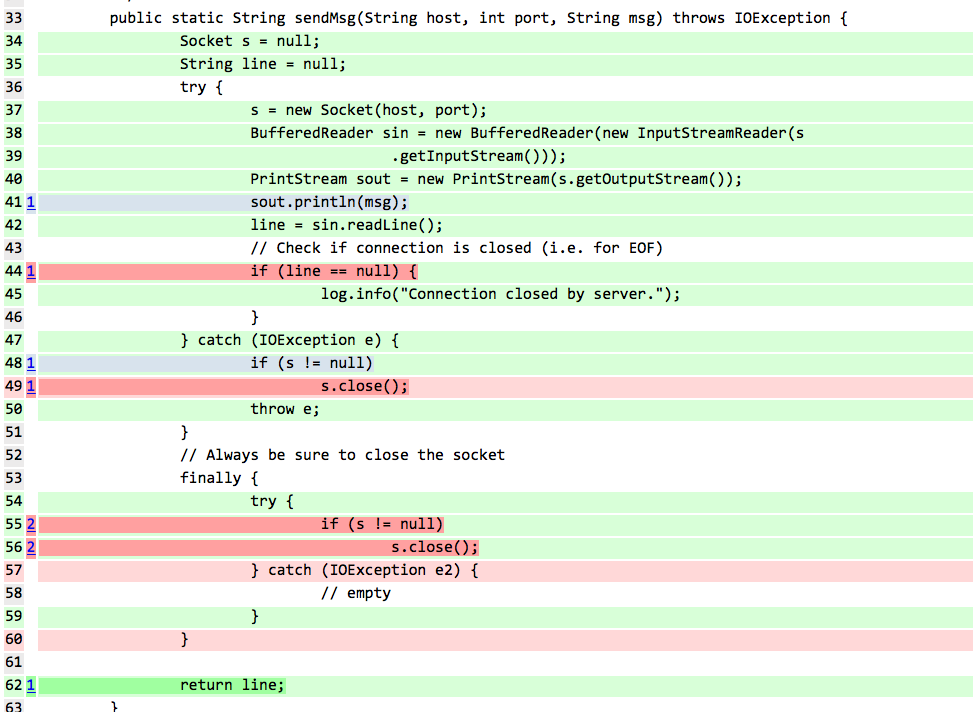
\includegraphics[width=.99\textwidth]{images/MutationTesting/sendMsgCode.png}
\end{center}
\caption{Code for the sendMsg method}
\label{fig:sendMsgCode}
\end{figure}

\begin{figure}[!htb]
\begin{center}
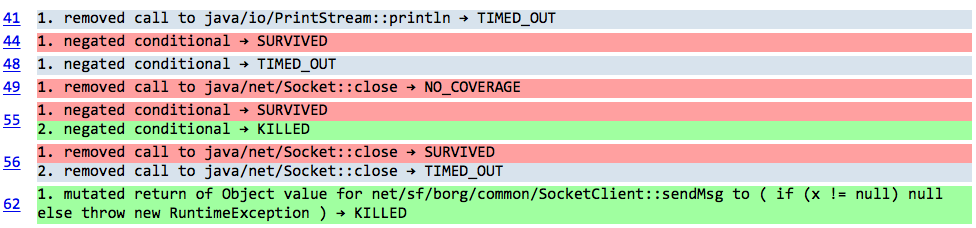
\includegraphics[width=.99\textwidth]{images/MutationTesting/sendMsgMutant.png}
\end{center}
\caption{Mutations for the sendMsg method}
\label{fig:sendMsgMutant}
\end{figure}

\clearpage
The results show that not all mutants have been killed. From Figure \ref{fig:sendMsgCode} we can see that our mutation testing results can be possibly improved if more tests on the server and socket state are created. 

\bigskip

\fontsize{14}{5}\textbf{After Additional Test Cases}

\begin{figure}[!htb]
\begin{center}
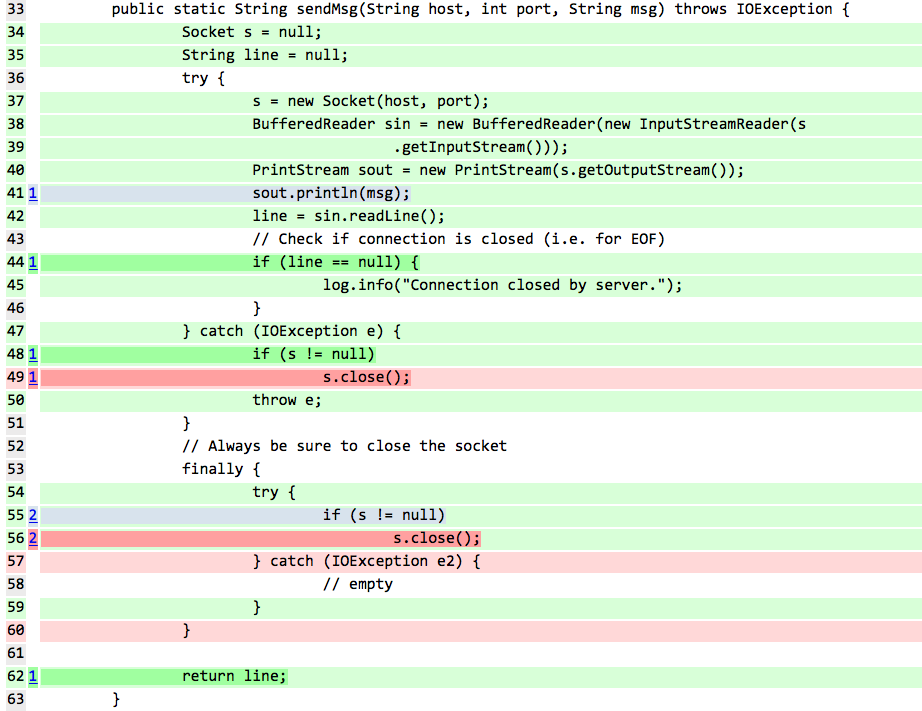
\includegraphics[width=.99\textwidth]{images/MutationTesting/sendMsgCodeAfter.png}
\end{center}
\caption{Updated code results for the sendMsg method}
\label{fig:sendMsgCodeAfter}
\end{figure}

\begin{figure}[!htb]
\begin{center}
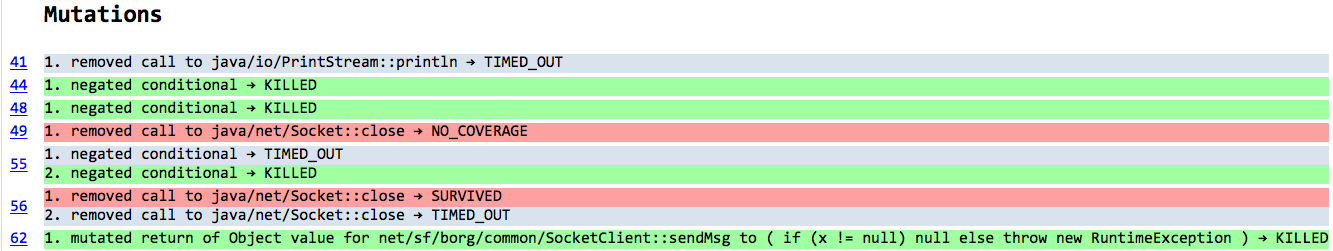
\includegraphics[width=.99\textwidth]{images/MutationTesting/sendMsgMutantAfter.png}
\end{center}
\caption{Updated mutations for the sendMsg method}
\label{fig:sendMsgMutantAfter}
\end{figure}

The test case shown below was added and improved results to what is shown in Figures \ref{fig:sendMsgCodeAfter} and \ref{fig:sendMsgMutantAfter}. This test case kills the mutant at lines 44, 48 without increasing line coverage. Thus, showing how test cases built for coverage alone are not sufficient. \\

The remaining bugs all relate to the \emph{close} function of the Socket object instantiated in the \emph{sendMsg} method. When Pitclipse mutates the \emph{close} function and removes it, this action causes a timeout. Which is why the \emph{sendMsg} method is defensively programmed to ensure that the socket connection is closed after the message is sent. Due to the amount of defensive programming and case of timeouts it is not possible to achieve full mutation testing coverage for this method consistently between all machines.

\begin{lstlisting}[caption={Additional test case for sendMsg},label={list:sendMsg}]
    @Test
    public void checkServerAlive() {
    String msg = null;
    SocketServer ss;
    String response;
        try {
            ss = new SocketServer(2922, this);
            response = SocketClient.sendMsg("localhost", 2922, msg);
            assertTrue(ss.isAlive());
        } catch (IOException e) {
            // TODO Auto-generated catch block
            e.printStackTrace();
        }
    }
\end{lstlisting}

\begin{itemize}
\item The data flow analysis you performed and the calculation of the coverage metrics. You must
show which test cases are responsible for which dc-paths.
\item A description of the test cases you added to improve coverage. If your coverage was already high,
discuss how your testing was able to achieve this.
\item The slices that you identified and the percentage of slices that your testing covers. You must
show which test cases are responsible for which slices.
\item A description of the test cases you added to improve slice coverage. If your coverage was
already high, discuss how your testing was able to achieve this.
\item Evaluate the effectiveness of your test cases using mutation testing. Discuss and address any
issues if you have found in your written report.
\item Attaching bug reports if bugs are discovered using your testing methods. You should use the
same bug report format as in Assignment 1. Do not file these bug reports to the project’s bug
report system.
\item An appendix with the specification of the methods you are testing
\end{itemize}

\section{JPetStore}

\begin{itemize}
\item The test scenarios that you have created;
\item The request rates and the duration of the load tests;
\item The analysis of your load tests and the description of any problems that you have found (if there
are any).
\end{itemize}

\end{document}
